\section{IPC tramite Binder}\label{sec:ipcbinder}
\begin{figure}[thp]
\centering
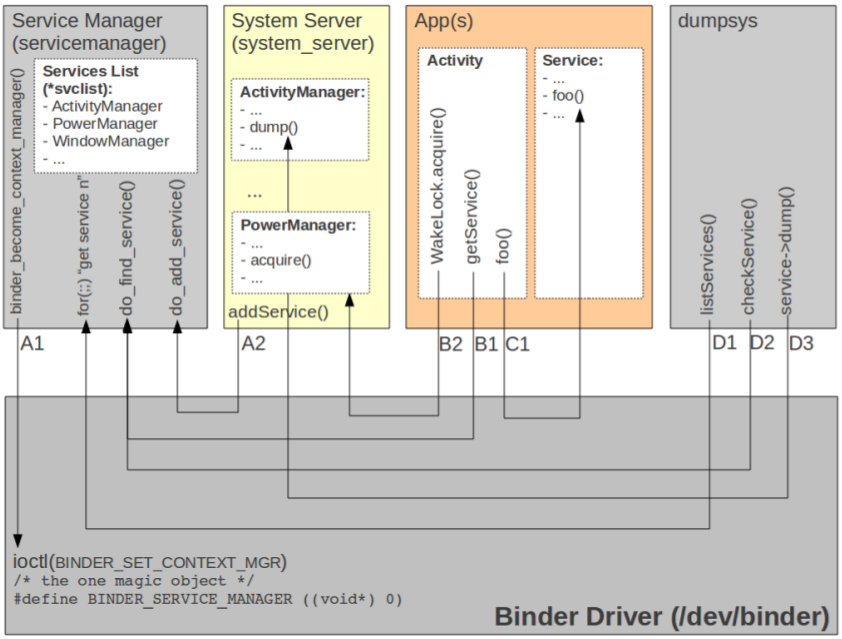
\includegraphics[scale=0.5]{img/embed/binder.png}
\caption{Alcuni meccanismi di IPC tramite \texttt{\small /dev/binder}. \parencite{libro:embedded}}
\label{fig:yagBinder}
\end{figure}

La maggior parte delle interazioni interessanti che avvengono all'interno di 
Android sono possibili grazie al Binder, implementazione Google di \textit{OpenBinder}
della \textit{Be Inc}, dove quest'ultima non è più supportata. Come riferiscono i primi
ideatori, questo è un «componente localizzato a livello
di sistema,  per fornire un'astrazione di alto livello al di sopra
dei tradizionali sistemi operativi». Andando ora nel dettaglio della corrente
implementazione, il Binder permette di effettuare IPC per chiamare metodi
remoti, in questo caso quello dei \textit{service}, come se fossero locali, utilizzando
un meccanismo di chiamate sincrone tramite meccanismi di richiesta e risposta:
ciò implica che, se il chiamato (es.) esegue un ciclo infinito senza fornire una
risposta, il chiamante rimarrebbe bloccato;
è stato tuttavia previsto un meccanismo di \textit{Death Notification}
grazie al quale il chiamante in attesa viene notificato della cessazione del
servizio remoto.

In particolare abbiamo che il \textit{Service Manager}, dopo essere stato
avviato nello\\
\texttt{\small init.rc} e dopo essersi registrato presso il Binder tramite l'invocazione
di \texttt{\small ioctl} con il comando \texttt{\small BINDER\_SET\_CONTEXT\_MGR}, acquisisce la possibilità
di diventare il \textit{Context Manager} di sistema, avendo  la possibilità
di fornire l'indicizzazione di tutti i \textit{service} di sistema. In
questo modo è in grado di fornire al richiedente l'istanza del Binder
di comunicazione, in modo da interagire con il servizio richiesto. Un esempio
pratico dell'utilizzo del \textit{Service Manager} è facilmente riscontrabile all'interno delle Java API, 
come nel caso dell'ottenimento del \texttt{NotificationManager}:
\begin{java}
NotificationManager mNotificationManager = (NotificationManager)getSystemService(Context.NOTIFICATION_SERVICE);
\end{java}

\begin{figure}[thp]
\centering
\subfloat[][\textit{Architettura \textit{High-level} della comunicazione tramite Binder lato Java. \parencite{tesi:binder}}]{\label{subfig:architecturebinder}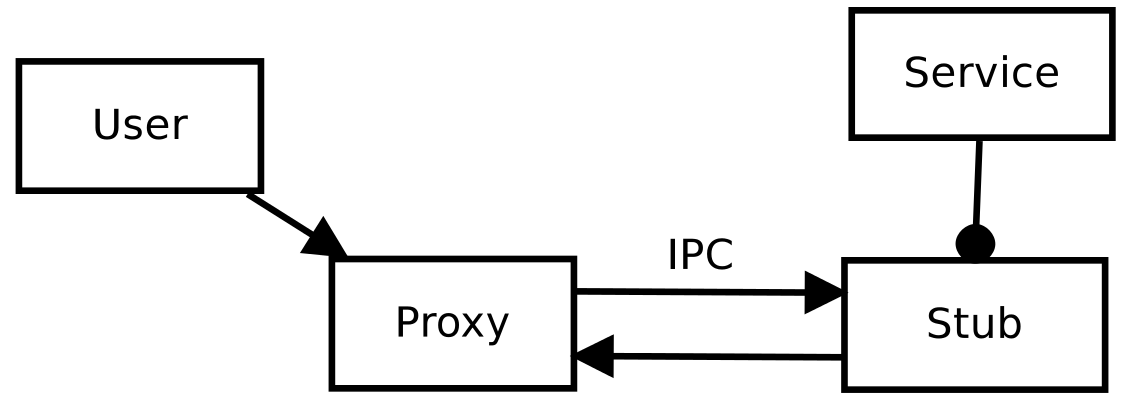
\includegraphics[scale=0.3]{img/teutonic_ipc.png}}\\
\subfloat[][\textit{Generalizzazione della gerarchia tra classi lato client e \textit{service}. \url{http://www.aesop.or.kr/Board_Documents_Android_Frameworks/34984}}]{\label{subfig:generalclassstub}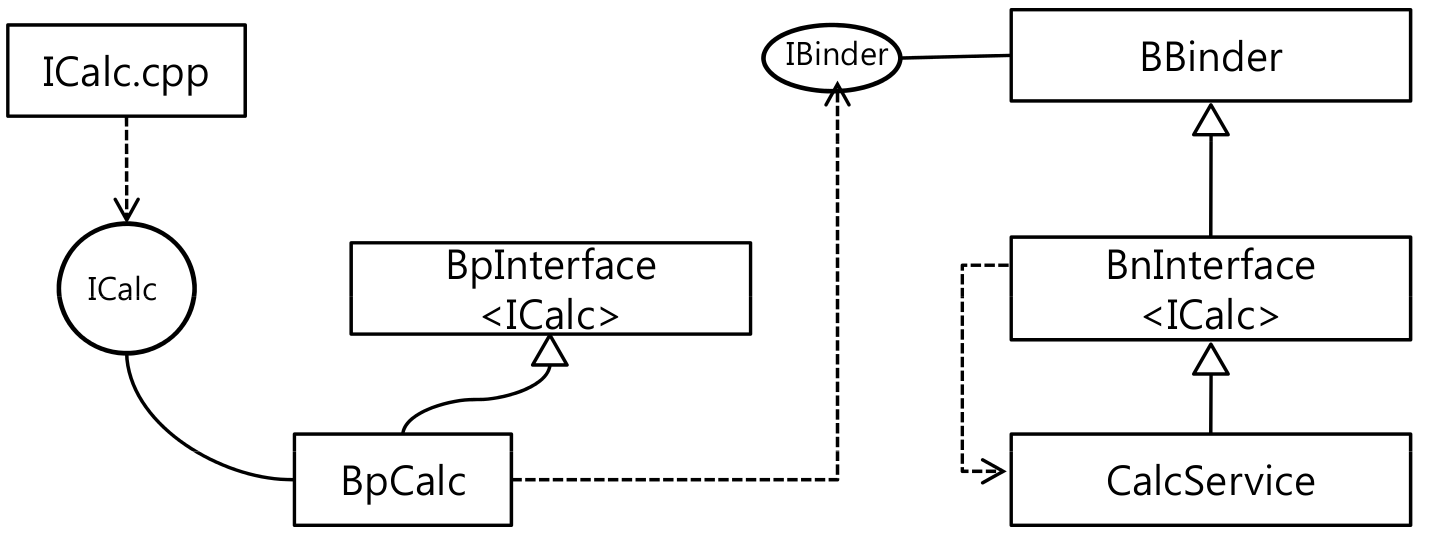
\includegraphics[scale=0.3]{img/korea/userproxystub.png}}\\
\caption{\textit{Overview} del protocollo di comunicazione predisposto dal Binder.}
\label{fig:androidbindhieroverview}
\end{figure}

Come possiamo vedere dalla Figura \subref{subfig:architecturebinder}
 \vref{fig:androidbindhieroverview}, l'applicazione client (nell'immagine \textit{User})
dispone di un \textit{proxy} di comunicazione che funge da tramite per
la comunicazione con lo \textit{stub} interagente con il \textit{service}: in genere nelle applicazioni del mondo Java
queste implementazioni sono fornite automaticamente dalla compilazione di
interfacce dette AIDL (\textsc{Android Interface Definition Language}) \parencite{libro:carli},
anche se possono essere esse stesse prodotte dallo stesso sviluppatore \parencite{tesi:binder}.

Questa forma di comunicazione è resa possibile sia dal fatto che 
\textit{proxy} e \textit{stub} hanno un'interfaccia  comune, sia perché
allo stesso \textit{proxy} viene fornita un'istanza del Binder tramite la quale viene
resa possibile la comunicazione IPC. Mostro inoltre di seguito un esempio di 
codice generato automaticamente dalla definizione della AIDL, del quale mi
interesserò unicamente della trattazione dello \textit{stub} lato \textit{service}.
\lstinputlisting[language=Java,caption= IPermissionController,label=lst:stubipermissioncontroller]{srcs/Stub.java}
Posso inoltre sottolineare come ad ogni \textit{service} sia associato un
descriptor, ovvero una stringa identificativa, che potrà essere utilizzata
da un client per richiedere un'istanza del \textit{proxy} tramite il quale
far avvenire la comunicazione.

\bigskip

All'interno della Sottosezione \vref{subsec:mischeWilhelm} mostrerò il meccanismo
di IPC che avviene a livello di librerie del sistema operativo, mentre mostrerò
molto brevemente nella Sottosezione \vref{subsub:ndkbuild} come sia possibile
compilare i files AIDL in codice Java.

